\documentclass{article}
\usepackage{graphicx} % Required for inserting images
\graphicspath{ {./images/} }

\title{MS-CS Course Note (Non-Credit Course 3)}
\author{Mark Zhou}
\date{July 2024}

\usepackage{setspace}
\usepackage{listings}
\usepackage{amssymb}
\usepackage{xcolor}
\usepackage{float}

\setlength{\intextsep}{1cm}

\begin{document}
\maketitle
\doublespacing

\paragraph{This is my course note on “Trees And Graphs: The Basics” provided by Colorado University of Boulder. 
This is a non-credit prep course for an MS-CS degree.}

\newpage
\tableofcontents
\newpage


\section{Binary Search Trees}

\subsection{Basic Concepts}

\paragraph{
    Binary search tree is a binary tree is a kind of data type with set of data elements without repeatition.\\
    We can insert, delete, search, and traverse the data elements in 
    a binary search tree.\\
    For each element in it, there will be a key of the element, which will 
    always be a number.\\
    With this setting in place, we can always comparing different elements 
    by comparing their keys, even if the elements are not numbers.\\
}

\paragraph{
    In the figure, we have a binary search tree with some nodes and 
    leaves. Every node has two children nodes and those leaves, which 
    have no children nodes, are called nil nodes.\\
    Every node has an element with a key, and the key of the left child
    node is always $<$ the key of the parent node, and the key of
    the right child node is always $>$ the key of the parent node.\\
    The left and right child nodes are also binary search trees.\\
    That is to say, the keys are always in a sorted order regardless of
    the structure of the tree. When we move the elements around, the keys 
    will be different for each elements, in order to remain in the sorted 
    order.\\
    The leaves have no elements.\\
}

\begin{figure}[H]
    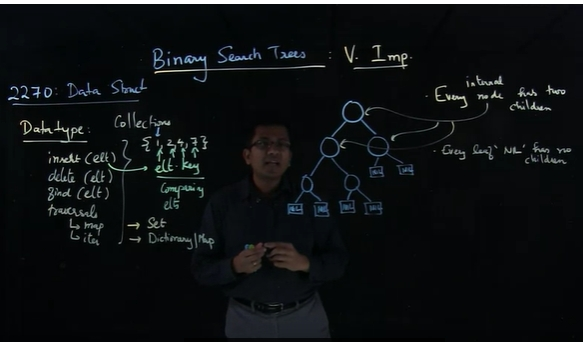
\includegraphics[width=\textwidth]{binarysearchtreenodes.png}
\end{figure}

\paragraph{
    When there is a node with the key 25, every node in the left subtree
    will have a key $<$ 25, and every node in the right subtree will
    have a key $>$ 25.\\
    The rule will also apply to all those subtrees.\\
}

\begin{figure}[H]
    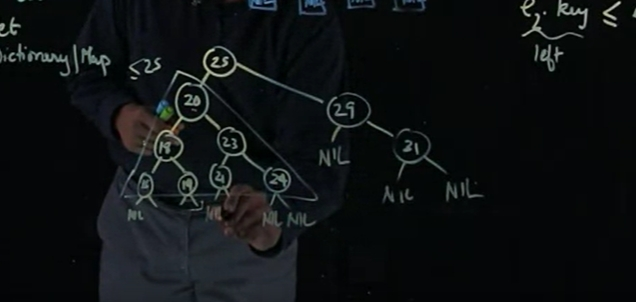
\includegraphics[width=\textwidth]{binarysearchtreerealexample.png}
\end{figure}

\begin{verbatim}
    Example:
     25
    /  \
   15  50
  / \  / \
 10 22 35 70
\end{verbatim}

\begin{verbatim}

Question:
Binary Search Trees may look similar to Heaps, but it is important 
to consider their differences.
In a Min-Heap, the smallest element must be the root node of the tree.
In a Binary Search Tree, on the other hand, how would we find the 
smallest element?

A: We would traverse the left subtree of the root node until we 
reach a leaf node, which means a node with a NIL as its left child.
\end{verbatim}


\subsection{The Height of a Binary Search Tree}

\paragraph{
    The height of a binary search tree is the number of edges on the
    longest path from the root node to a leaf node.\\
    We will define the height of a leaf node as 0. Then the height of number 25, 
    a.k.a. the root node of the below binary search tree is 2.\\
}

\newpage

\begin{verbatim}
    Example:
     25       -> height = 2
    /  \
   15  50     -> height = 1
  / \  / \
 10 22 35 70  -> height = 0, since they are leaf nodes
\end{verbatim}

\paragraph{
    Let's assume we have a balanced binary search tree with n internal nodes.\\
    One each layer from the root node, there'll be $2^0$ nodes, $2^1$ nodes, $2^2$ nodes, $\cdots$, $2^h$ nodes.\\
    The total number of nodes in the tree will be $2^0+2^1+2^2+ \cdots +2^h=2^{h+1}-1$.\\
    So, the height of the tree will be $h=\log_2(n+1)-1$.\\
    In the sense of big O notation, the height of a binary search tree is $O(\log_2(n))$, in a balanced binary 
    search tree scenario.\\
    For example, $\log_2^8=3$, so the height of a binary search tree with 8 nodes is 3.\\
    $\log_2^{15}=4$, so the height of a binary search tree with 15 nodes is 4.\\
}

\paragraph{
    In the worst case scenario, where the binary search tree is not balanced, the height of the tree will be $O(n)$.\\
    That is to say, the tree will be a linked list looks like this;\\
}

\newpage

\begin{verbatim}
    Linked List Example:
     10
      \
       15
        \
         20
          \
           25
            \
             30
              \
               35
\end{verbatim}

\paragraph{
    In this case, the height of the tree is 6, which is equal to the number of nodes in the tree.\\
    The height of the tree is $O(n)$, which is the worst case scenario.\\
    Normally, we will have something in between the best case scenario and the worst case scenario, 
    $O(\log(n)) < height < O(n)$.\\
}

\subsection{Basics of Binary Search Tree Quiz}

\begin{figure}[H]
    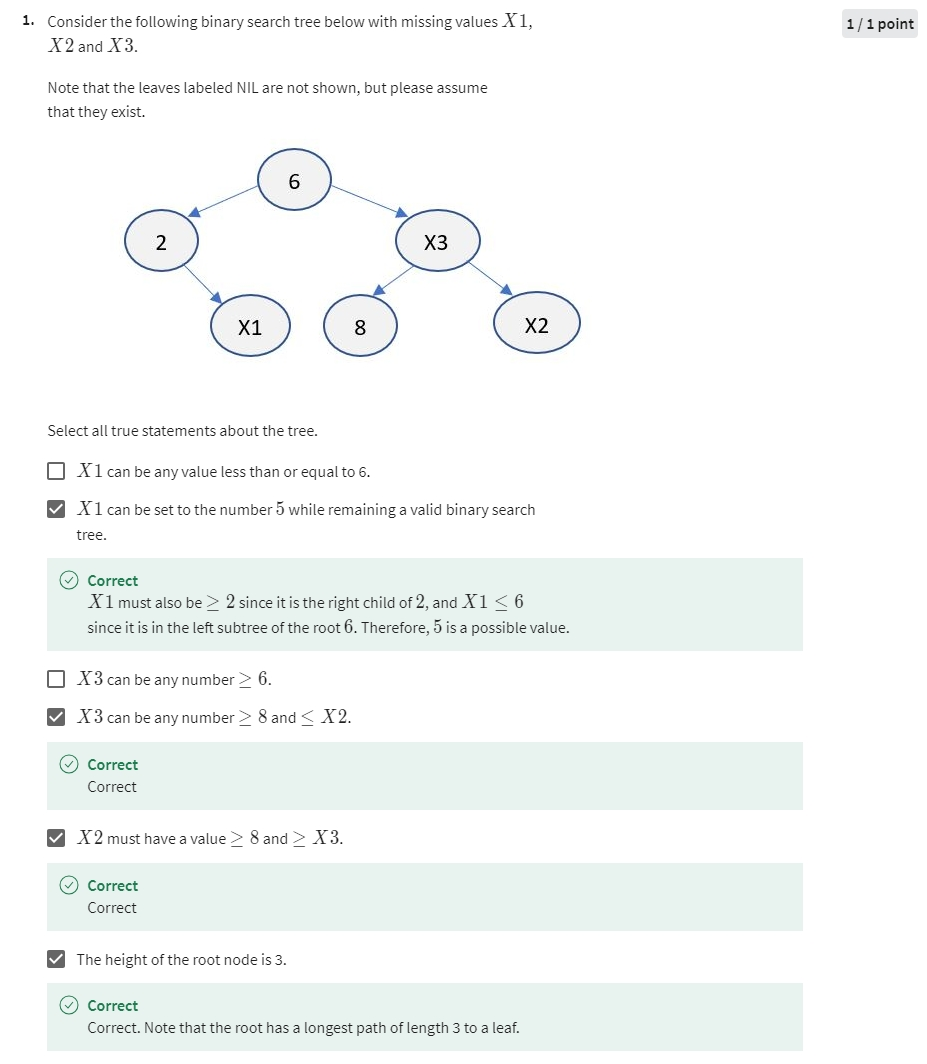
\includegraphics[width=\textwidth]{binarysearchtreequiz01.png}
\end{figure}

\begin{figure}[H]
    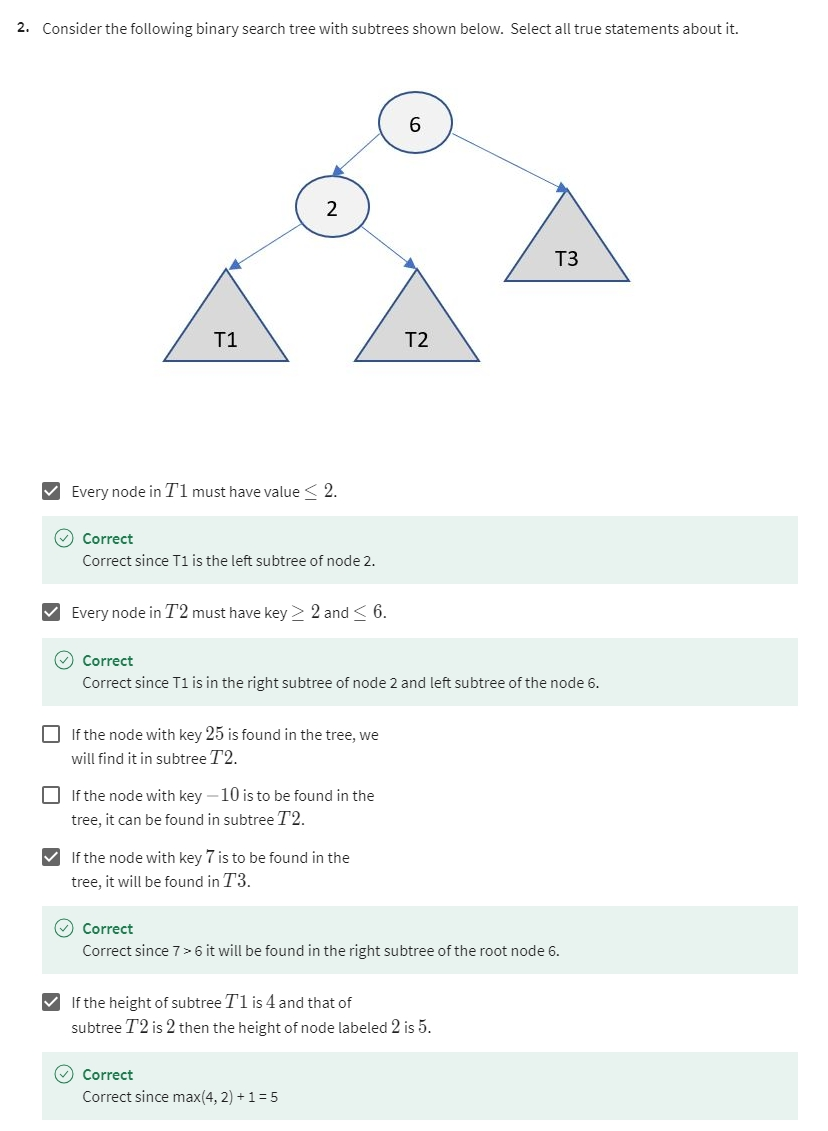
\includegraphics[width=\textwidth]{binarysearchtreequiz02.png}
\end{figure}

\begin{figure}[H]
    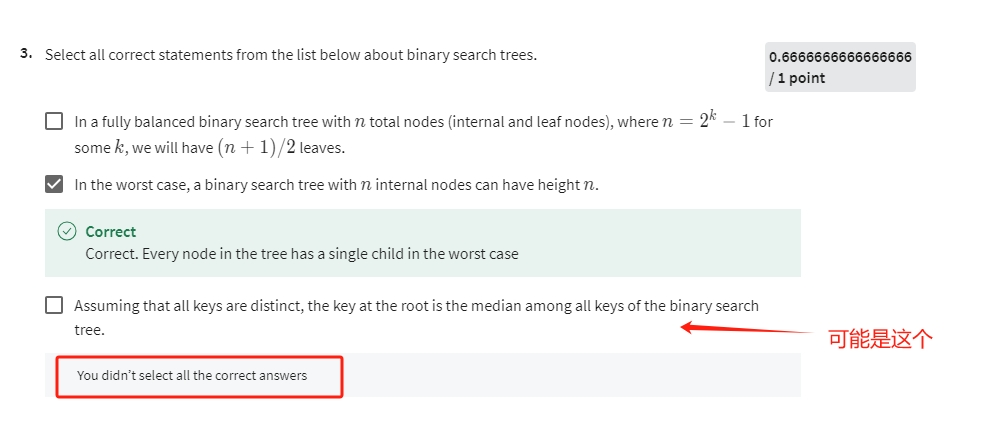
\includegraphics[width=\textwidth]{binarysearchtreequiz03.png}
\end{figure}



\subsection{Insertion and Deletion in a Binary Search Tree}

\paragraph{
    We can insert a new element into a binary search tree by comparing the key of the new element with the key of the root node.\\
    If the key of the new element is less than the key of the root node, we will insert the new element into the left subtree.\\
    If the key of the new element is greater than the key of the root node, we will insert the new element into the right subtree.\\
    We will repeat the process until we reach a leaf node.\\
}

\paragraph{
    For example, we have a binary search tree with the following nodes;\\
}

\begin{verbatim}
    Example:
     25
    /  \
   15  50
  / \  / \
 10 22 35 70
\end{verbatim}

\paragraph{
    If we want to insert a new element with the key 40, we will compare 40 with 25, and then 40 with 50, and then 40 with 35.\\
    Since 40 is greater than 35, we will insert 40 as the right child node of 35.\\
}





TBC: Binary search tree: insertion and deletion video.


\end{document}